% Shock Engine institutional dossier, version 2.0.
% Composed by research/dossier/build-dossier.ts, which writes numbers.tex (figures read from the
% published research files) and data/ (figure series) next to this file before compiling.
% Figures typed here come from the Markdown reports listed in Appendix B.
\documentclass[11pt,a4paper]{article}

% ------------------------------------------------------------------ packages
\usepackage[T1]{fontenc}
\usepackage[utf8]{inputenc}
\usepackage[english]{babel}
\usepackage{mathpazo}
\usepackage{tgpagella}
\usepackage[scale=0.92]{tgheros}
\usepackage[a4paper,top=2.7cm,bottom=2.5cm,left=2.5cm,right=2.5cm,headheight=15pt,headsep=0.8cm]{geometry}
\usepackage{microtype}
\usepackage{amsmath,amssymb}
\usepackage{array,booktabs,tabularx,threeparttable,multirow}
\usepackage[table]{xcolor}
\usepackage{tikz}
\usetikzlibrary{positioning,arrows.meta,calc,fit,backgrounds,decorations.pathreplacing}
\usepackage{pgfplots}
\pgfplotsset{compat=1.18}
\usepgfplotslibrary{fillbetween}
\usepackage[skins,breakable]{tcolorbox}
\usepackage{enumitem}
\usepackage{float}
\usepackage{needspace}
\usepackage{etoolbox}
\usepackage{titletoc}
\usepackage{fancyhdr}
\usepackage{lastpage}
\usepackage{titlesec}
\usepackage[font=small,labelfont={bf,sf},labelsep=period,margin=0pt]{caption}
\usepackage[authoryear,round]{natbib}
\usepackage{xurl}
\usepackage[colorlinks=true,linkcolor=navy,citecolor=navy,urlcolor=navy,
  pdftitle={Shock Engine: Institutional Dossier},pdfauthor={Oreste Raynaud},
  pdfsubject={Strategy, execution and capacity of a systematic intraday strategy on Bitcoin and Ether},
  pdfkeywords={Shock Engine, execution, implementation shortfall, market impact, capacity, Bitcoin, Ether}]{hyperref}

\input{numbers.tex}

% ------------------------------------------------------------------ colours and styles
\definecolor{navy}{RGB}{16,42,84}
\definecolor{accent}{RGB}{0,122,110}
\definecolor{ink}{RGB}{30,34,40}
\definecolor{muted}{RGB}{105,114,125}
\definecolor{hair}{RGB}{205,211,218}
\definecolor{soft}{RGB}{242,245,248}
\definecolor{warm}{RGB}{252,246,236}
\definecolor{amber}{RGB}{176,108,18}
\definecolor{good}{RGB}{46,125,70}
\definecolor{bad}{RGB}{178,46,46}
\definecolor{greyline}{RGB}{150,156,164}
\AtBeginDocument{\color{ink}}

\setlength{\parskip}{4pt}
\setlength{\parindent}{0pt}
\renewcommand{\arraystretch}{1.18}
\setlist{itemsep=3pt,topsep=4pt,leftmargin=1.4em}
\setlist[itemize]{label={\color{accent}\small$\blacktriangleright$}}

\titleformat{\section}{\sffamily\LARGE\bfseries\color{navy}}{\color{accent}\thesection}{0.6em}{}
\titlespacing*{\section}{0pt}{18pt}{8pt}
\titleformat{\subsection}{\sffamily\large\bfseries\color{navy}}{\thesubsection}{0.6em}{}
\titlespacing*{\subsection}{0pt}{12pt}{4pt}
\pretocmd{\section}{\needspace{14\baselineskip}}{}{}
\pretocmd{\subsection}{\needspace{8\baselineskip}}{}{}
\titlecontents{section}[1.7em]{\vspace{2pt}\sffamily\small\bfseries\color{navy}}{\contentslabel{1.7em}}{\hspace*{-1.7em}}{\hfill\contentspage}
\titleformat{\paragraph}[runin]{\sffamily\bfseries\color{navy}}{}{0pt}{}[.]

\pagestyle{fancy}
\fancyhf{}
\fancyhead[L]{\sffamily\scriptsize\color{muted}SHOCK ENGINE\quad\textbullet\quad INSTITUTIONAL DOSSIER}
\fancyhead[R]{\sffamily\scriptsize\color{muted}VERSION 2.0\quad\textbullet\quad 12 OCTOBER 2026}
\fancyfoot[L]{\sffamily\scriptsize\color{muted}Oreste Raynaud\quad\textbullet\quad ShadowMarketPro Research}
\fancyfoot[R]{\sffamily\scriptsize\color{muted}\thepage\,/\,\pageref*{LastPage}}
\renewcommand{\headrulewidth}{0.4pt}
\renewcommand{\headrule}{\hbox to\headwidth{\color{hair}\leaders\hrule height \headrulewidth\hfill}}

\newtcolorbox{keybox}[1][]{enhanced,breakable,colback=soft,colframe=navy,boxrule=0pt,leftrule=2.5pt,arc=0pt,
  left=9pt,right=9pt,top=6pt,bottom=6pt,before skip=8pt,after skip=8pt,
  fonttitle=\sffamily\bfseries\small,coltitle=navy,colbacktitle=soft,titlerule=0pt,toptitle=5pt,bottomtitle=-2pt,title={#1}}
\newtcolorbox{discbox}[1][]{enhanced,breakable,colback=warm,colframe=amber,boxrule=0pt,leftrule=2.5pt,arc=0pt,
  left=9pt,right=9pt,top=6pt,bottom=6pt,before skip=8pt,after skip=8pt,
  fonttitle=\sffamily\bfseries\small,coltitle=amber,colbacktitle=warm,titlerule=0pt,toptitle=5pt,bottomtitle=-2pt,title={#1}}
\newtcolorbox{casebox}[1][]{enhanced,breakable,colback=white,colframe=accent,boxrule=0.6pt,arc=1pt,
  left=9pt,right=9pt,top=6pt,bottom=6pt,before skip=8pt,after skip=8pt,
  fonttitle=\sffamily\bfseries\small,coltitle=white,colbacktitle=accent,title={#1}}

% The allocator's question that opens a section.
\newcommand{\question}[1]{\par\vspace{-2pt}{\sffamily\itshape\color{accent}#1}\par\vspace{6pt}}
\newcommand{\bps}{\,bps}
\newcommand{\minus}{\textminus}
\newcolumntype{L}{>{\raggedright\arraybackslash}X}
\newcolumntype{R}{>{\raggedleft\arraybackslash}X}
\newcommand{\thead}[1]{{\sffamily\bfseries\footnotesize #1}}

\pgfplotsset{
  dossier/.style={
    width=\linewidth, axis lines*=left, axis line style={hair}, tick style={hair},
    tick label style={font=\sffamily\scriptsize,text=muted}, label style={font=\sffamily\footnotesize,text=muted},
    legend style={font=\sffamily\scriptsize,draw=none,fill=none}, grid=major, grid style={hair!60},
    every axis plot/.append style={line join=round}},
}

\begin{document}

% ================================================================== cover
\begin{titlepage}
\thispagestyle{empty}
\begin{tikzpicture}[remember picture,overlay]
  \fill[navy] (current page.north west) rectangle ([yshift=-11.2cm]current page.north east);
  \fill[accent] ([yshift=-11.2cm]current page.north west) rectangle ([yshift=-11.45cm]current page.north east);
  \node[anchor=north west,inner sep=0,text=white!80!navy,font=\sffamily\scriptsize\bfseries]
    at ([xshift=2.5cm,yshift=-2.1cm]current page.north west)
    {QUANTITATIVE RESEARCH\quad\textbullet\quad INSTITUTIONAL DOSSIER\quad\textbullet\quad VERSION 2.0};
  \node[anchor=north west,inner sep=0,text=white,font=\sffamily\bfseries\fontsize{42}{46}\selectfont]
    at ([xshift=2.45cm,yshift=-3.1cm]current page.north west) {Shock Engine};
  \node[anchor=north west,inner sep=0,text=white,font=\sffamily\Large,text width=14.5cm,align=left]
    at ([xshift=2.5cm,yshift=-5.2cm]current page.north west)
    {Strategy, execution and capacity of a systematic intraday strategy on Bitcoin and Ether};
  \node[anchor=north west,inner sep=0,text=white!80!navy,font=\sffamily\small,text width=14.5cm,align=left]
    at ([xshift=2.5cm,yshift=-7.0cm]current page.north west)
    {Eight years of simulated trading, all 2{,}474 executions since 2020 replayed on real market data,
     and an honest account of what remains to be proven.};
  \node[anchor=north west,inner sep=0,text=white,font=\sffamily\normalsize]
    at ([xshift=2.5cm,yshift=-9.4cm]current page.north west)
    {\textbf{Oreste Raynaud}\quad\textbullet\quad ShadowMarketPro Research\quad\textbullet\quad 12 October 2026};
\end{tikzpicture}

\vspace*{10.6cm}

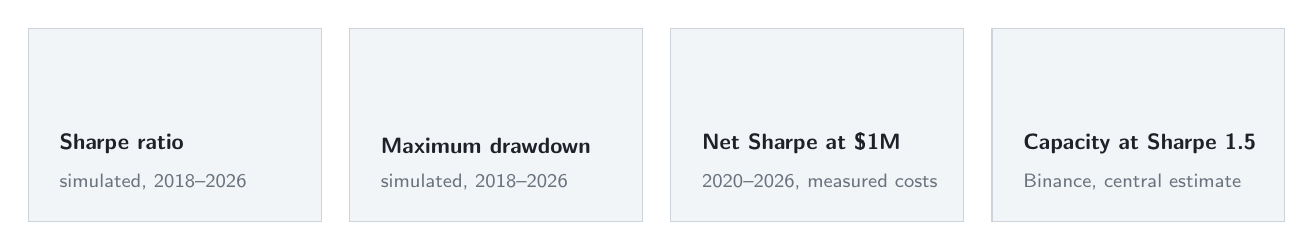
\begin{tikzpicture}[tile/.style={draw=hair,fill=soft,minimum width=3.72cm,minimum height=2.45cm,inner sep=0}]
  \foreach \i/\v/\l/\s in {
      0/{\PfSharpe}/{Sharpe ratio}/{simulated, 2018--2026},
      1/{\PfMaxDD}/{Maximum drawdown}/{simulated, 2018--2026},
      2/{\ShDeliveredOne}/{Net Sharpe at \$1M}/{2020--2026, measured costs},
      3/{\CapDelivered}/{Capacity at Sharpe 1.5}/{Binance, central estimate}} {
    \node[tile] (t\i) at (\i*4.08cm,0) {};
    \node[anchor=north west,font=\sffamily\bfseries\fontsize{22}{24}\selectfont,text=navy] at ([xshift=8pt,yshift=-8pt]t\i.north west) {\v};
    \node[anchor=south west,font=\sffamily\footnotesize\bfseries,text=ink,align=left] at ([xshift=8pt,yshift=21pt]t\i.south west) {\l};
    \node[anchor=south west,font=\sffamily\scriptsize,text=muted,align=left] at ([xshift=8pt,yshift=8pt]t\i.south west) {\s};
  }
\end{tikzpicture}

\vspace{0.9cm}

{\sffamily\small
\begin{tabularx}{\textwidth}{@{}>{\bfseries\color{navy}}p{3.4cm}L@{}}
Status of the evidence & In-sample historical simulation after commissions, with execution costs measured on real
  Binance market data. A pre-registered forward test started on 12~October~2026. \textbf{There is no live track record on real
  capital yet.}\\[3pt]
What is inside & The strategy and how it was tested; a framework for executing large notional drawn from the market-impact
  literature; the 2{,}474 executions; costs, capacity and forward-looking estimates; what we got wrong; risks.\\
\end{tabularx}}

\vfill
{\sffamily\scriptsize\color{muted}
Historical simulation after modelled and measured transaction costs. Not live performance. Simulated results have inherent
limitations and benefit from hindsight in the design of the rules. Past simulated performance does not predict future results.
This document is neither investment advice nor an offer of any financial product or service. Proprietary thresholds, window
lengths and exit multiples are not disclosed; no test reported here depends on knowing them.\par}
\end{titlepage}

% ================================================================== foreword
\section*{A note before the numbers}
\addcontentsline{toc}{section}{A note before the numbers}

Every systematic strategy begins as a story the data seems to tell. Shock Engine's story is simple: when Bitcoin or Ether
moves abnormally within fifteen minutes, and the move is confirmed by its surroundings, it tends to keep going for a few hours.
The backtest says this story has paid well for eight years.

We have learned to distrust that sentence. A backtest is a hypothesis about the past, written by someone who already knew how
the past ended. So this dossier is organised around the questions an allocator asks \emph{after} reading the headline Sharpe
ratio. Would the strategy have survived real execution? How much capital can it carry before its own orders eat the edge?
What would prove it wrong, and when will we know?

We tried to answer them the way a careful trading desk would. For the validation studies, we wrote each test down before running it. We measured with
market data rather than assumptions, and when a convenient model and a measurement disagreed, we kept the measurement. We
tried hard to break our own result. And we say plainly, throughout, which numbers are \emph{demonstrated}, which are
\emph{estimated}, and which only live trading can settle.

We were wrong several times along the way: about a three-second wait nobody had measured, about how much market impact to
expect, about the cost of trading Ether, and even about a figure in the first draft of this very document. Those corrections
are collected in Section~\ref{sec:wrong}, because how a team handles its mistakes says more about its process than any single
figure.

What this document does not contain is a live track record on real capital. That is the next chapter. It will be reported from
its own start date, separately from the simulation, whatever it shows.

\vspace{6pt}
{\sffamily\bfseries\color{navy}Oreste Raynaud}\\
{\sffamily\small\color{muted}ShadowMarketPro Research, 12 October 2026}

\vspace{14pt}
{\sffamily\small
\renewcommand{\contentsname}{\sffamily\large\bfseries\color{navy}Contents}
\setcounter{tocdepth}{1}
\tableofcontents}

\newpage
% ================================================================== summary
\section*{At a glance}
\addcontentsline{toc}{section}{At a glance}

Shock Engine is a systematic intraday strategy on Bitcoin and Ether. Over 1~September~2018 to 30~September~2026 its
50/50 portfolio shows, in simulation, a Sharpe ratio of \PfSharpe{} and a maximum drawdown of \PfMaxDD{}, against \BhSharpe{}
and \BhMaxDD{} for buy-and-hold. The result survives placebos, delays, parameter perturbations, a transfer to Ether and a
regression on standard trend strategies. Replaying all 2{,}474 historical executions on real market data, with the bot as it is
now coded, the net Sharpe at \$1M of capital over 2020--2026 is estimated at \ShDeliveredOne{} (\BtSharpe{} before execution
costs) and stays above 1.5 up to about \CapDelivered{} on Binance. The evidence remains in-sample, the intended venue (Hyperliquid) has thinner books than Binance, and
there is no live track record yet.

\begin{table}[H]
\centering\small
\begin{tabularx}{\textwidth}{@{}>{\raggedright\arraybackslash}p{0.315\textwidth}>{\raggedright\arraybackslash}p{0.315\textwidth}>{\raggedright\arraybackslash}X@{}}
\toprule
{\sffamily\bfseries\color{good}Demonstrated} {\sffamily\scriptsize\color{muted}(data, reproducible)} &
{\sffamily\bfseries\color{amber}Estimated} {\sffamily\scriptsize\color{muted}(model, conditional)} &
{\sffamily\bfseries\color{bad}Open} {\sffamily\scriptsize\color{muted}(needs live trading)}\\
\midrule
The historical edge is not drift, exit shape or a knife-edge parameter: random entries lose to it 100\% of the time, every
perturbed neighbour is profitable.
& Net Sharpe at \$1M: \ShDeliveredOne{} [\ShLoDeliveredOne; \ShHiDeliveredOne], CAGR \CagrDeliveredOne{}, funding excluded.
& Persistence out of sample. A walk-forward on Bitcoin keeps a Sharpe of 1.11, against 1.49 for the fixed rules.\\[4pt]
It is not repackaged trend following: residual alpha \RaAlpha{} a year, $t=\RaT$, against six standard trend strategies
(in-sample).
& Capacity at Sharpe 1.5: about \CapDelivered{} on Binance (central estimate, wide interval).
& The short-entry condition (E2), specified after the data were studied: a pre-registered forward test, about three years.\\[4pt]
All 2{,}474 executions replayed on real trades: 89\% of market orders demonstrably fillable at \$1M, none shown unfillable.
& On Hyperliquid: about \$1.9M if its books are half as deep as Binance's; about \$0.45M at the depth visible on Bitcoin.
& Our own market impact; Hyperliquid depth beyond 20 levels; the bot's real latency on its server.\\[4pt]
Each second of delay costs money: \DriftHalf\bps{} at 0.5\,s, \DriftFive\bps{} at 5\,s after the signal.
& Cost of the bot as now coded (not yet deployed or traded) at \$1M: \CostMeanDeliveredOne\bps{} per execution, \BudgetDeliveredOne{} of
  the budget compatible with a Sharpe of 1.5.
& A live track record. One year cannot reliably tell a Sharpe of 1.5 from zero (Section~\ref{sec:forward}).\\
\bottomrule
\end{tabularx}
\end{table}

\begin{keybox}[How to read the numbers in this dossier]
\textbf{Simulated} means a historical replay of fixed rules. \textbf{Measured} means observed in historical market data (real
trades and order books), not orders sent by Shock Engine. \textbf{Estimated} means a model fitted to those measurements.
Strategy figures cover 2018--2026; execution figures cover 2020--2026, the period with Binance perpetual futures. All costs are
in basis points (bps) of the traded notional; Sharpe ratios are annualised from daily returns unless stated otherwise.
\end{keybox}

\newpage
% ================================================================== 1. method
\section{How we worked: the scientific approach}\label{sec:method}
\question{``Why should I believe any of this?''}

The headline numbers are strong, which is precisely why they deserve suspicion. Searching many rules on one history inflates
in-sample performance \citep{white2000,bailey2014,harvey2016}. We cannot remove that bias after the fact, but we can bound it,
expose it and test around it. Six working rules shaped everything that follows.

\begin{enumerate}[label={\sffamily\bfseries\color{accent}\arabic*.},leftmargin=1.6em]
\item \textbf{Write the test before running it.} The validation studies of the last phase were pre-registered (Table~\ref{tab:prereg}):
  hypothesis, statistic, thresholds and data were committed to version control before the first computation, in the tradition
  of clinical trials \citep{nosek2018}. The commit is the timestamp. The earlier robustness tests of Table~\ref{tab:robust} used
  criteria set during the original research, without a committed protocol.
\item \textbf{Try to break the result, not to confirm it.} Random-entry placebos, delayed entries, shifted regimes and
  synthetic markets ask whether something with no edge could have done as well.
\item \textbf{Measure before modelling.} When a measurement and a convenient model disagreed, we kept the measurement and
  reported the gap. Section~\ref{sec:wrong} shows how often this mattered.
\item \textbf{Never use the future.} Every simulated decision uses only information available at that instant: closed
  candles, the order book as it stood, the previous day's regime.
\item \textbf{Separate demonstrated, estimated and open.} A number's status travels with it, all the way to the summary.
\item \textbf{Publish failures and corrections.} Markets where the rules fail, tests that came out against us, and our own
  errors are reported next to the successes.
\end{enumerate}

\begin{figure}[H]
\centering
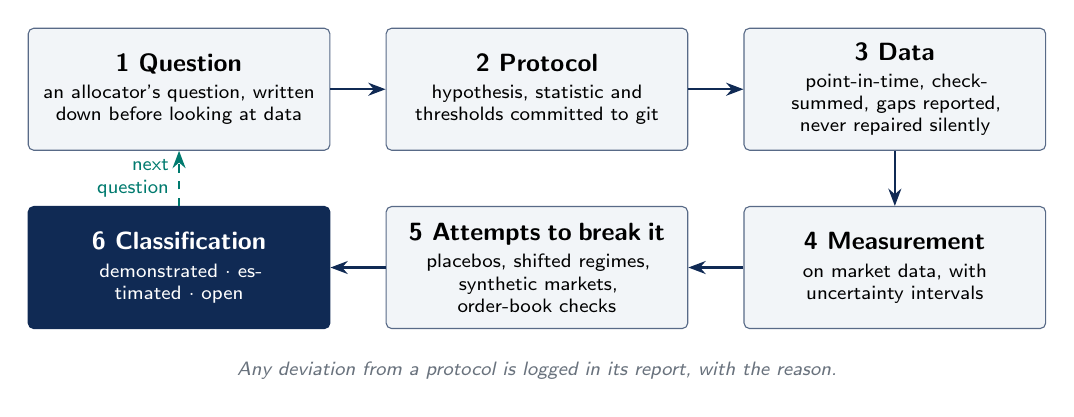
\begin{tikzpicture}[node distance=7mm and 7mm,
  box/.style={draw=navy!70,fill=soft,rounded corners=2pt,text width=3.55cm,align=center,font=\sffamily\scriptsize,minimum height=1.55cm,inner sep=4pt},
  arr/.style={-{Stealth[length=2.2mm]},navy,thick}]
  \node[box] (q) {{\bfseries\small 1\,\,Question}\\[2pt]an allocator's question, written down before looking at data};
  \node[box,right=of q] (p) {{\bfseries\small 2\,\,Protocol}\\[2pt]hypothesis, statistic and thresholds committed to git};
  \node[box,right=of p] (d) {{\bfseries\small 3\,\,Data}\\[2pt]point-in-time, checksummed, gaps reported, never repaired silently};
  \node[box,below=of d] (m) {{\bfseries\small 4\,\,Measurement}\\[2pt]on market data, with uncertainty intervals};
  \node[box,left=of m] (f) {{\bfseries\small 5\,\,Attempts to break it}\\[2pt]placebos, shifted regimes, synthetic markets, order-book checks};
  \node[box,left=of f,fill=navy,text=white,draw=navy] (c) {{\bfseries\small 6\,\,Classification}\\[2pt]demonstrated $\cdot$ estimated $\cdot$ open};
  \draw[arr] (q) -- (p); \draw[arr] (p) -- (d); \draw[arr] (d) -- (m); \draw[arr] (m) -- (f); \draw[arr] (f) -- (c);
  \draw[arr,dashed,accent] (c.north) -- node[left,font=\sffamily\scriptsize,text=accent,align=right]{next\\question} (q.south);
  \node[font=\sffamily\scriptsize\itshape,text=muted,below=3mm of f] {Any deviation from a protocol is logged in its report, with the reason.};
\end{tikzpicture}
\caption{The research cycle behind every study in this dossier.}
\label{fig:cycle}
\end{figure}

\paragraph{The evidence ladder} Not all evidence is equal. Table~\ref{tab:ladder} ranks what each kind of test can rule out
and where Shock Engine stands on each rung. The honest summary is that the strategy has climbed the rungs that history allows
and is now on the ones that only time can climb.

\begin{table}[H]
\centering\small
\caption{The evidence ladder: what each kind of test rules out, and where Shock Engine stands.}
\label{tab:ladder}
\begin{tabularx}{\textwidth}{@{}c>{\raggedright\arraybackslash}p{3.7cm}L>{\raggedright\arraybackslash}p{4.1cm}@{}}
\toprule
\thead{Rung} & \thead{Evidence} & \thead{What it rules out} & \thead{Shock Engine}\\
\midrule
1 & In-sample simulation after costs & Nothing on its own & Sharpe \PfSharpe{}, 2018--2026\\
2 & Placebos, delays, parameter neighbourhoods & Market drift, exit artefacts, knife-edge parameters & Passed (Table~\ref{tab:robust})\\
3 & Transfer to markets never used for design & Fitting the noise of one price series & Ether passed on two feeds; Solana, gold, TAO failed\\
4 & Walk-forward re-selection & Look-ahead in the choice of parameters & Bitcoin: 1.11 against 1.49\\
5 & Execution replay on real market data & The illusion of frictionless fills & 2{,}474 executions, Sections~\ref{sec:fills}--\ref{sec:capacity}\\
6 & Pre-registered forward test & Hindsight in the rules themselves & Running since 12 Oct.~2026\\
7 & Live track record on real capital & All of the above, plus our own impact & \textbf{Not yet available}\\
\bottomrule
\end{tabularx}
\end{table}

\paragraph{Pre-registered studies} Pre-registration was adopted for the validation phase. The strategy rules themselves were
developed earlier without it, which is why every historical performance figure in this dossier is treated as in-sample.
Table~\ref{tab:prereg} lists the protocols; their commit hashes are in Appendix~\ref{app:sources}.

\begin{table}[H]
\centering\small
\caption{Pre-registered studies, in the order their protocols were committed.}
\label{tab:prereg}
\begin{tabularx}{\textwidth}{@{}>{\raggedright\arraybackslash}p{1.5cm}>{\raggedright\arraybackslash}p{3.5cm}L>{\raggedright\arraybackslash}p{4.3cm}@{}}
\toprule
\thead{Committed (2026)} & \thead{Study} & \thead{Question} & \thead{Outcome}\\
\midrule
8 Oct. & Short entries, 8 unseen assets & Do symmetric filters improve the short side? & Improvement not demonstrated ($p=0.44$)\\
8 Oct. & E2 forward test & Do shorts in a bearish regime beat the others? & Running since 12 Oct.~2026\\
8 Oct. & E2 historical diagnostics & Can past data eliminate the E2 condition? & Not eliminated; not a validation\\
9 Oct. & E2 falsification (tests A--C) & Is E2's historical gain exceptional? & Short quality: yes. Sharpe gain: largely generic\\
9 Oct. & Residual alpha & Is it repackaged trend following? & No: alpha \RaAlpha{}/yr, $t=\RaT$ (in-sample)\\
12 Oct. & Capacity, phases P0--P1 & What cost can the strategy bear? & Budget of \BudgetBps\bps{} per execution at Sharpe 1.5\\
12 Oct. & Latency drift & What does each second of delay cost? & \DriftFive\bps{} at 5\,s, \DriftHalf\bps{} at 0.5\,s\\
12 Oct. & Executability, \$500k and \$1M & Could every order have been filled, and at what price? & 95\% and 89\% demonstrated; none shown unfillable\\
\bottomrule
\end{tabularx}
\end{table}

% ================================================================== 2. strategy
\section{The strategy}\label{sec:strategy}
\question{``What exactly is being traded, and does the edge survive scrutiny?''}

\subsection{Economic intuition}
Two views compete about what follows a large price move. Under \emph{underreaction}, information is absorbed gradually and
prices drift in the direction of the move \citep{hongstein1999}. Under \emph{overreaction} or liquidity provision, the move is
partly a temporary concession that reverts. Which dominates is an empirical question, and the answer may depend on the state of
the market. Shock Engine bets on continuation, but only after the move has been qualified: shocks are measured against local
volatility, in the spirit of nonparametric jump tests \citep{leemykland2008}, and their clustering reflects the self-exciting
dynamics documented for jumps. The short side is conditioned on the market state because momentum payoffs are state dependent
and crash in rebounds \citep{danielmoskowitz2016}.

\subsection{The rules, in words}
\begin{itemize}
\item \textbf{Signal.} A 15-minute return that is extreme relative to local volatility and breaks the recent range.
\item \textbf{Qualification.} Higher-timeframe trend on the right side, a candle that closes near its extreme, abnormal
  volume, shocks that cluster, and a calm enough volatility state before the shock.
\item \textbf{Regimes.} One rule set for calm markets, one for agitated markets, read from the last closed day.
\item \textbf{Exits.} A volatility-scaled initial stop, a partial take-profit, a trailing stop, an exit on a moving reference
  price, or a qualified shock in the opposite direction.
\item \textbf{Short side (specification E2).} A mirror of the long side, admitted only when the daily trend regime is bearish.
\item \textbf{Exposure.} One position per market at a time, 100\% of that market's capital, no leverage, no pyramiding, no
  averaging down. The portfolio holds half of the capital in each market and never rebalances.
\item \textbf{Calibration.} Rules set on Bitcoin only and applied unchanged to Ether.
\end{itemize}

\begin{discbox}[Disclosure: the short-entry condition was specified after the data were studied]
During development the short side was an unconditional mirror of the long side (version v1). The trend condition that defines
specification E2 was introduced on 8~October~2026, as an exploratory variant of a pre-registered study, after the 2017--2026
data had been examined. Every historical figure in this dossier is therefore in-sample with respect to it. Without the
condition, the same portfolio shows a Sharpe ratio of 1.73, a CAGR of 64.5\% and a maximum drawdown of \minus23.5\% over the
same period. Three pre-registered falsification tests (Table~\ref{tab:robust}) find the improvement in the quality of shorts
exceptional, but most of the gain in Sharpe ratio and drawdown generic. Only the forward test of Section~\ref{sec:forward} can
validate it.
\end{discbox}

\subsection{Historical results}

\begin{figure}[H]
\centering
\begin{tikzpicture}
\begin{axis}[dossier, height=6.2cm, ymode=log, log basis y=10, ymin=40, ymax=12000,
    ytick={100,1000,10000}, yticklabels={100,1{,}000,10{,}000}, xmin=2018.6, xmax=2026.85, xticklabels={},
    ylabel={Value of 100 (log scale)}, legend pos=north west, name=eq]
  \addplot[navy, thick] table[x=x,y=pf]{data/equity.dat};
  \addlegendentry{Shock Engine portfolio 50/50}
  \addplot[greyline, semithick] table[x=x,y=bh]{data/equity.dat};
  \addlegendentry{Buy-and-hold BTC/ETH 50/50}
\end{axis}
\begin{axis}[dossier, height=3.6cm, at={(eq.south west)}, anchor=north west, yshift=-0.25cm,
    xmin=2018.6, xmax=2026.85, ymin=-0.8, ymax=0, ytick={-0.75,-0.5,-0.25,0},
    yticklabels={\minus75\%,\minus50\%,\minus25\%,0\%}, xtick={2019,2020,2021,2022,2023,2024,2025,2026},
    x tick label style={/pgf/number format/1000 sep=}, ylabel={Drawdown}]
  \addplot[greyline, semithick, fill=greyline!25] table[x=x,y=bh]{data/drawdown.dat} \closedcycle;
  \addplot[navy, semithick, fill=navy!30] table[x=x,y=pf]{data/drawdown.dat} \closedcycle;
\end{axis}
\end{tikzpicture}
\caption{Value of 100 invested and drawdown from the running peak, daily closes, 1~September~2018 to 30~September~2026.
Historical simulation after commissions; buy-and-hold without costs.}
\label{fig:equity}
\end{figure}

\begin{table}[H]
\centering\small
\begin{threeparttable}
\caption{Simulated performance, 1~September~2018 to 30~September~2026.}
\label{tab:headline}
\begin{tabular}{@{}lrrrr@{}}
\toprule
& \thead{Portfolio 50/50} & \thead{Bitcoin} & \thead{Ether} & \thead{Buy-and-hold}\\
\midrule
Sharpe ratio & \textbf{\PfSharpe} & \BtcSharpe & \EthSharpe & \BhSharpe\\
CAGR & \PfCagr & 41.0\% & 72.2\% & \BhCagr\\
Annualised volatility & \PfVol & 25.8\% & 34.3\% & 69.0\%\\
Maximum drawdown & \PfMaxDD & \minus22.3\% & \minus26.8\% & \BhMaxDD\\
Sortino ratio & \PfSortino & 3.18 & 4.04 & --\\
Calmar ratio & \PfCalmar & 1.84 & 2.70 & 0.44\\
\midrule
Trades (long / short) & \Trades{} (\TradesLong{} / \TradesShort) & 644 & 667 & --\\
Win rate; average win / average loss & \WinRate; \Payoff & 32\%; 4.00 & 30\%; 4.68 & --\\
Time in market & \TimeInMarket & 16\% & 18\% & 100\%\\
\bottomrule
\end{tabular}
\begin{tablenotes}[flushleft]\footnotesize
\item Daily UTC close-to-close returns, annualised with $\sqrt{365.25}$, zero risk-free rate. Commission 0.045\% per order;
no slippage, funding or leverage. Bitcoin and Ether columns are the two halves of the portfolio, each on its own capital.
\end{tablenotes}
\end{threeparttable}
\end{table}

The two strategies are much less correlated (\CorrDaily) than the coins themselves (0.82): each is out of the market most of
the time. Split in two halves, the portfolio Sharpe ratio is \HalfOne{} and then \HalfTwo{}. The rolling one-year Sharpe ratio
is positive in \RollPositive{} of windows and above one in \RollAboveOne. A month-block bootstrap gives a 90\% interval of
\BootLo{} to \BootHi{}; a bootstrap resamples history and is not a forecast. The worst calendar month lost \WorstMonth.

The profile is convex: the strategy wins \WinRate{} of its trades, and its average winner is \Payoff{} times its average loser.
The best 5\% of trades account for \TopFive{} of the portfolio's log growth; without them the CAGR would be \CagrNoTopFive.
Missing a handful of large moves in live trading would change the outcome materially, which is why execution reliability,
not only execution cost, matters so much here.

\subsection{Robustness}

\begin{table}[H]
\centering\small
\caption{Tests designed to break the result. Placebo, delay and transfer criteria come from the original research and were applied
unchanged; walk-forward and neighbourhood results are descriptive; the three E2 tests were pre-registered.}
\label{tab:robust}
\begin{tabularx}{\textwidth}{@{}>{\raggedright\arraybackslash}p{5.1cm}L@{}}
\toprule
\thead{Test} & \thead{Result}\\
\midrule
Random entries with identical exits (200 runs) & The strategy beats 100\% of runs on Bitcoin and on Ether (criterion: 95\%).\\
Every entry delayed by one bar & 83\% (Bitcoin) and 94\% (Ether) of the average trade kept.\\
Transfer without recalibration & Ether passes on two independent feeds (Sharpe 1.84 Binance, 1.87 Dukascopy). Solana (0.35),
  gold (\minus0.07) and TAO (\minus0.01) fail.\\
All parameters perturbed jointly by $\pm$20\% (300 neighbours) & Every neighbour profitable; median Sharpe 1.32 (Bitcoin), 1.77
  (Ether). On Bitcoin the chosen set sits at the top of its neighbourhood, on Ether in the middle: a plateau, not a peak.\\
Walk-forward, Bitcoin, 28 quarterly windows 2020--2026 & Sharpe 1.11 against 1.49 for the fixed rules; maximum drawdown
  \minus34.9\%. Part of the headline result is a selection effect.\\
Regression on buy-and-hold and six trend strategies & Residual alpha \RaAlpha{} a year, Newey--West $t=\RaT$;
  \RaUnexplained{} of the mean return unexplained \citep{neweywest1987}.\\
E2 falsification, test A: random selection of shorts & Quality of shorts kept: 96.8th percentile ($p=0.032$). Portfolio
  Sharpe: $p=0.055$.\\
E2 falsification, test B: shifted regimes & $p=0.005$ for the portfolio, $0.093$ for Bitcoin alone, $0.001$ for Ether.\\
E2 falsification, test C: synthetic markets & Short quality above the synthetic 95th percentile at every block length; the
  Sharpe gain only at the 43rd to 78th percentile.\\
\bottomrule
\end{tabularx}
\end{table}

Sharpe ratios in the transfer, neighbourhood and walk-forward rows are annualised from 15-minute returns and differ slightly from the daily
figures. The rules are not a universal law of markets: they work on the two most liquid crypto assets and fail elsewhere, and
we see no reason to hide it.

% ================================================================== 3. framework
\section{Executing large notional: what the literature tells us}\label{sec:framework}
\question{``A backtest fills at the close. What would a real \$1M order have paid?''}

A backtest assumes that each order is filled at the closing price of the bar that triggered it. A real order arrives later,
crosses a spread, consumes liquidity and may move the price for the next one. Before measuring anything we fixed the vocabulary,
borrowed from four decades of research on institutional execution.

\subsection{Implementation shortfall}
\citet{perold1988} defined the cost of trading as the gap between a ``paper'' portfolio, executed at the decision price, and the
real one. For an order of side $s=\pm1$, decided at price $P_d$ (here the close used by the backtest), arriving at $t_a$ when the
mid-price is $m_{t_a}$ and the best quote on our side is $q_{t_a}$, and filled at an average price $\bar P$:
\begin{equation}
\mathrm{IS}
= \underbrace{s\,\frac{m_{t_a}-P_d}{P_d}}_{\text{delay: drift before arrival}}
+ \underbrace{s\,\frac{q_{t_a}-m_{t_a}}{P_d}}_{\text{half-spread}}
+ \underbrace{s\,\frac{\bar P-q_{t_a}}{P_d}}_{\text{depth: walking the book}} .
\label{eq:is}
\end{equation}
Every cost in Sections~\ref{sec:fills}--\ref{sec:capacity} is measured in these three parts, in basis points, separately from
exchange fees, which the backtest already pays once per order.

\subsection{Urgency against impact}
\citet{almgrenchriss2000} framed optimal execution as a trade-off: trading slowly reduces impact but exposes the order to price
risk. When the order is driven by a short-lived signal, the price risk has a sign: the market moves \emph{with} the signal, and
waiting costs the edge itself \citep{cartea2015}. For a schedule of duration $T$, the expected cost is roughly
\begin{equation}
\mathbb{E}[C(T)] \approx D(T) + I(Q,T),
\label{eq:urgency}
\end{equation}
where $D$, the drift during execution, grows with $T$ and $I$, the impact of quantity $Q$, shrinks with $T$. Shock Engine sits
at the urgent extreme. At its signal times the price moves against a waiting order by \DriftHalf\bps{} in half a second and
\DriftFive\bps{} in five seconds (Figure~\ref{fig:drift}); spreading the order over the next minute costs 4.6\bps{} (Bitcoin)
and 6.9\bps{} (Ether) of drift. Taking the visible book at once costs a fraction of that, at the median, up to \$2.5M orders on
the rebuilt books (Section~\ref{sec:costs}). The optimal schedule collapses to a single immediate order, and engineering latency, not
order slicing, is where the money is.

\subsection{The square-root law, and why it overstated our costs}
The best-documented regularity in market impact is the square-root law: a metaorder of size $Q$, executed incrementally,
moves the price by about
\begin{equation}
I(Q) \approx Y\,\sigma_D\,\sqrt{Q/V_D},
\label{eq:sqrt}
\end{equation}
where $\sigma_D$ is daily volatility, $V_D$ daily volume and $Y$ a constant of order one \citep{toth2011,bouchaud2018},
including on Bitcoin \citep{donierbonart2015}. Estimated exponents vary: about 0.6 on US equities in \citet{almgren2005}, a
logarithmic shape in \citet{zarinelli2015}. Our first capacity study, pre-registered, used Equation~\eqref{eq:sqrt} with $Y\in\{0.5,1,2\}$
because no calibration was available. It implied about 3\bps{} for a \$500k order in the central case.

The median measured cost of the first \$500k of real orders of that size at our signal times was 0.30\bps{} on Bitcoin and
0.72\bps{} on Ether. The two numbers measure different things. The square-root law describes metaorders spread over minutes to days,
including the reaction of liquidity providers to repeated flow. A single marketable order that sweeps the book in
milliseconds pays the shape of the book at that instant \citep{obizhaevawang2013,cont2014}, and the books of Bitcoin and Ether
perpetuals are deep near the touch. \citet{frazzini2018}, using a large manager's live executions, also found real costs well
below model-based estimates. We take the measurement, with one caveat that the order-book check in Section~\ref{sec:costs}
confirms: large real orders tend to arrive when liquidity is there, so a method built on them can flatter the cost of an order
sent at a fixed time.

\subsection{Capacity, two venues, and what remains unmeasured}
\begin{itemize}
\item \textbf{Capacity.} Studies of anomalies measure how trading costs erode returns as size grows
  \citep{novymarxvelikov2016,landier2015,frazzini2018}. We define capacity as the capital at which the net Sharpe ratio falls
  below 1.5, a threshold fixed in the pre-registered protocol, not chosen after seeing the curve.
\item \textbf{Two venues, one price?} Crypto prices can differ persistently across exchanges \citep{makarovschoar2020}. Signals
  are computed on Bitstamp and Binance spot data, costs are measured on Binance perpetuals, and the bot trades Hyperliquid
  perpetuals. We measure the cross-venue gap separately from book quality.
\item \textbf{Not measured.} Permanent impact and its decay \citep{gatheral2010,bacry2015}, and the reaction of market makers
  to a predictable flow at 15-minute closes. Only our own live fills can measure them.
\end{itemize}

% ================================================================== 4. fills
\section{The 2{,}474 executions}\label{sec:fills}
\question{``Could every order have been filled, and at what price?''}

Every execution of the portfolio from January 2020 to September 2026, without exception, was replayed on the real trades of
Binance USD-M perpetual futures, the most liquid venue and the only one with free millisecond trade history
covering the period. None is demonstrably unfillable at \$500k or \$1M of capital.

\begin{table}[H]
\centering\small
\begin{threeparttable}
\caption{The executions studied, January 2020 to September 2026.}
\label{tab:counts}
\begin{tabular}{@{}lrrrl@{}}
\toprule
\thead{Type} & \thead{Bitcoin} & \thead{Ether} & \thead{Total} & \thead{Order used by the bot}\\
\midrule
Entries & 541 & 556 & 1{,}097 & marketable limit (IOC)\\
Exits at the close & 103 & 118 & 221 & marketable limit (IOC)\\
Stops and trailing stops & 438 & 438 & 876 & stop triggered by the exchange\\
Partial take-profits (TP1) & 126 & 154 & 280 & resting limit\\
\midrule
\textbf{Total} & \textbf{1{,}208} & \textbf{1{,}266} & \textbf{2{,}474} & \\
\bottomrule
\end{tabular}
\begin{tablenotes}[flushleft]\footnotesize
\item By year: 1{,}165 executions in 2020--2022, 338 in 2023, 368 in 2024, 338 in 2025 and 265 from January to September 2026.
\end{tablenotes}
\end{threeparttable}
\end{table}

\paragraph{Data} 1{,}226 days of trades time-stamped to the millisecond from Binance's public archives, every file checked
against its published SHA-256 checksum, none unreadable. The reference price and, for the 876 stops, the moment the stop level
was crossed were found for 100\% of executions. Binance's book-depth snapshots ($\pm$1\%, since 2023) complement the trades, with
snapshots frozen for more than 30 minutes excluded. For 13 executions falling on free data days, the full Binance order book
was rebuilt to the millisecond (Section~\ref{sec:costs}).

\paragraph{Method: what an order of our size actually paid} Rather than assume an impact model, we looked for real orders of
our size around each execution (Figure~\ref{fig:method}). Aggressive orders were rebuilt from trades sharing a millisecond and
a side. When a real order of at least $Q$ dollars traded within two minutes of our arrival, the cost of its first $Q$ dollars is
what an order of our size really paid within two minutes of ours. When none did, the cost comes from a model fitted to these observations
($\log$ cost on size, volatility and volume; $R^2$ of 0.43 for Bitcoin and 0.32 for Ether; size elasticity 0.84 and 0.72).

\begin{figure}[H]
\centering
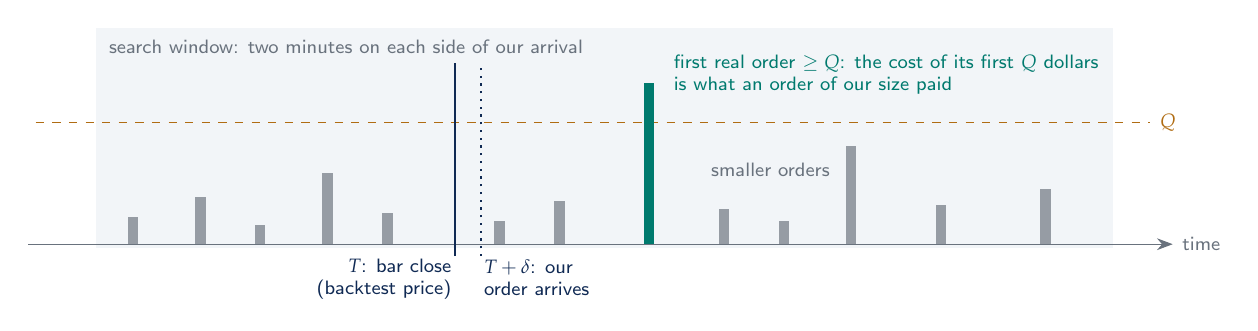
\begin{tikzpicture}[x=0.95cm,y=1cm,font=\sffamily\scriptsize]
  \fill[soft] (1.2,-0.05) rectangle (14.8,2.75);
  \node[anchor=north west,text=muted] at (1.25,2.72) {search window: two minutes on each side of our arrival};
  \draw[-{Stealth[length=2mm]},muted] (0.3,0) -- (15.6,0) node[right]{time};
  \draw[dashed,amber] (0.4,1.55) -- (15.3,1.55) node[right,text=amber]{$Q$};
  \foreach \x/\h in {1.7/0.35,2.6/0.6,3.4/0.25,4.3/0.9,5.1/0.4,6.6/0.3,7.4/0.55,9.6/0.45,10.4/0.3,11.3/1.25,12.5/0.5,13.9/0.7}
    \fill[greyline] (\x-0.07,0) rectangle (\x+0.07,\h);
  \fill[accent] (8.53,0) rectangle (8.67,2.05);
  \draw[navy,thick] (6.0,-0.15) -- (6.0,2.3);
  \node[below left,text=navy,align=right,inner sep=1pt] at (6.0,-0.15) {$T$: bar close\\(backtest price)};
  \draw[navy,thick,dotted] (6.35,-0.15) -- (6.35,2.3);
  \node[below right,text=navy,align=left,inner sep=1pt] at (6.35,-0.15) {$T+\delta$: our\\order arrives};
  \node[anchor=west,text=accent,align=left] at (8.8,2.15) {first real order $\geq Q$: the cost of its first $Q$ dollars\\is what an order of our size paid};
  \node[anchor=west,text=muted] at (9.3,0.95) {smaller orders};
\end{tikzpicture}
\caption{Measuring execution cost from comparable real orders. Grey bars are aggressive orders rebuilt from Binance trades,
with height proportional to size.}
\label{fig:method}
\end{figure}

\begin{table}[H]
\centering\small
\begin{threeparttable}
\caption{Reconciliation of the 2{,}194 market executions (entries, exits at the close, stops).}
\label{tab:reconcile}
\begin{tabular}{@{}lrrrr@{}}
\toprule
& \multicolumn{2}{c}{\thead{\$500k capital (\$250k orders)}} & \multicolumn{2}{c}{\thead{\$1M capital (\$500k orders)}}\\
\cmidrule(lr){2-3}\cmidrule(l){4-5}
\thead{Category, mutually exclusive} & \thead{Count} & \thead{Share} & \thead{Count} & \thead{Share}\\
\midrule
Comparable real order, first $Q$ dollars within 50\bps & 2{,}087 & 95.1\% & 1{,}957 & 89.2\%\\
Depth within 1\% only (book snapshots) & 2 & 0.1\% & 19 & 0.9\%\\
No direct evidence; cost estimated by the model & 105 & 4.8\% & 218 & 9.9\%\\
\midrule
Total & 2{,}194 & 100\% & 2{,}194 & 100\%\\
\bottomrule
\end{tabular}
\begin{tablenotes}[flushleft]\footnotesize
\item 50\bps{} is the price cap of the bot's market orders at entries and exits at the close; stops are exchange stop orders,
capped at 5\% from their trigger. Most executions without a comparable order are Ether in 2020--2022 (95
of 105 at \$500k; 174 of 218 at \$1M), when real orders of that size were rare. At \$2M of capital, 74\% of market executions
are demonstrated within 50\bps; at \$5M, 6\%, because \$2.5M orders exceed the largest size observed directly. All 280
take-profits were traded through (median excess 32\bps{} on Bitcoin, 35\bps{} on Ether); counting the 15 that cleared by less
than 5\bps{} as unfilled moves the Sharpe ratio from 1.838 to 1.835.
\end{tablenotes}
\end{threeparttable}
\end{table}

\begin{figure}[H]
\centering
\begin{tikzpicture}
\begin{axis}[dossier, height=5.4cm, ybar=2pt, bar width=13pt, ymin=0, ymax=112, ytick={0,25,50,75,100},
    yticklabel={\pgfmathprintnumber{\tick}\%}, xtick=data, xticklabels={\$250k,\$500k,\$1M,\$2M},
    enlarge x limits=0.18, xlabel={Order size}, ylabel={Share of market executions},
    nodes near coords={\pgfmathprintnumber[fixed,precision=0]{\pgfplotspointmeta}\%},
    every node near coord/.append style={font=\sffamily\tiny,text=ink},
    legend style={at={(0.98,0.98)},anchor=north east}, grid=none, ymajorgrids]
  \addplot[fill=navy,draw=none] table[x expr=\coordindex,y=btc]{data/census.dat};
  \addlegendentry{Bitcoin}
  \addplot[fill=accent!70,draw=none] table[x expr=\coordindex,y=eth]{data/census.dat};
  \addlegendentry{Ether}
\end{axis}
\end{tikzpicture}
\caption{How often a real aggressive order of at least our size traded within two minutes of a Shock Engine execution, by
order size. After our arrival, the first real \$500k order traded a median 7.4\,s later on Bitcoin and 14\,s later on Ether:
the book absorbs our size at once; we would not have to wait for other trades.}
\label{fig:census}
\end{figure}

% ================================================================== 5. costs
\section{Execution costs: measurement and control}\label{sec:costs}
\question{``Where does the money go between the signal and the fill?''}

The dominant cost is time, not size. With the bot as it is now built, a \$1M portfolio pays on average
\CostMeanDeliveredOne\bps{} per execution relative to the backtest price, \BudgetDeliveredOne{} of the budget compatible with a
Sharpe ratio of 1.5.

\paragraph{The cost budget} Adding one basis point of cost to every execution removes 0.064 from the Sharpe ratio. The
ratio stays above 1.5 as long as the average added cost stays below \BudgetBps\bps{} per execution (90\% interval: 0 to
14.5\bps, because the history itself is uncertain), and above 1.0 up to 13.1\bps.
Entries and stops carry the sensitivity; take-profits and exits at the close very little.

\begin{figure}[H]
\centering
\begin{tikzpicture}
\begin{axis}[dossier, height=6cm, xmin=0, xmax=10.3, ymin=-0.5, ymax=10.5, xtick={0,0.5,1,2,3,4,5,7,10},
    xticklabels={0,0.5,1,2,3,4,5,7,10}, xlabel={Seconds after the bar close}, ylabel={Adverse drift (bps)},
    legend style={at={(0.02,0.98)},anchor=north west}]
  \addplot[name path=hi, draw=none, forget plot] table[x=s,y=hi]{data/drift.dat};
  \addplot[name path=lo, draw=none, forget plot] table[x=s,y=lo]{data/drift.dat};
  \addplot[navy!14, forget plot] fill between[of=hi and lo];
  \addplot[navy, thick, mark=*, mark size=1.4pt] table[x=s,y=mean]{data/drift.dat};
  \addlegendentry{Mean drift against a waiting order (95\% interval)}
  \addplot[accent, dashed, semithick, domain=0:10.3, samples=2] {1.09};
  \addlegendentry{Depth cost of a \$1M order, Ether (book, median)}
  \addplot[greyline, dashed, semithick, domain=0:10.3, samples=2] {0.28};
  \addlegendentry{Depth cost of a \$1M order, Bitcoin (book, median)}
  \node[pin={[pin distance=8mm,font=\sffamily\scriptsize,text=navy,align=left]80:{delivered bot\\target: 0.5\,s}},
    circle,fill=navy,inner sep=1.6pt] at (axis cs:0.5,\DriftHalf) {};
  \node[pin={[pin distance=9mm,font=\sffamily\scriptsize,text=bad,align=left]-30:{initial bot:\\measured 5.0\,s}},
    circle,fill=bad,inner sep=1.6pt] at (axis cs:5,\DriftFive) {};
\end{axis}
\end{tikzpicture}
\caption{One second of delay costs more than sweeping a million dollars of book depth. Mean drift of the last traded price
against the order after the signal's bar close, \DriftN{} executions drawn at random and measured on Binance trades (pre-registered,
bootstrap 95\% interval). Depth costs: median over 13 rebuilt order books.}
\label{fig:drift}
\end{figure}

\paragraph{Latency, measured and engineered} The first strategy trade of the bot on Hyperliquid's test network carries an exchange
time stamp 5.01\,s after the bar close. Reading the code explained it: a fixed three-second wait, then seven to nine network
round trips made one after the other. Without touching the signals, the code was rewritten to read the closed candle as soon
as the exchange opens the next one, to run its network calls in parallel and to keep connections warm, leaving two round trips
between the close and the order. In the replay, this moves the Sharpe ratio at \$1M up by \GainDelivered{}
[\GainDeliveredLo; \GainDeliveredHi], positive in \GainDeliveredShare{} of paired bootstrap draws. The rewrite was committed on
12~October~2026; it is not yet confirmed deployed and has not traded. The 0.5\,s target is the optimistic end of the 0.5 to
0.9\,s expected from a server in Europe (0.1 to 0.3\,s from Tokyo); the new time stamps journalled by the bot will measure it.

\begin{table}[H]
\centering\small
\begin{threeparttable}
\caption{Execution cost per execution relative to the backtest price, exchange fees excluded (bps; Binance, 2020--2026).}
\label{tab:costs}
\begin{tabular}{@{}lrrrrr@{}}
\toprule
\thead{Capital, version of the bot} & \thead{Median} & \thead{P95} & \thead{P99} & \thead{Mean} & \thead{Share of budget}\\
\midrule
\$500k, initial bot (order at $T+5$\,s) & \CostMedCurrentHalf & \CostNinetyFiveCurrentHalf & \CostNinetyNineCurrentHalf & \CostMeanCurrentHalf & \BudgetCurrentHalf\\
\$500k, delivered bot (entries at $T+0.5$\,s) & \CostMedDeliveredHalf & \CostNinetyFiveDeliveredHalf & \CostNinetyNineDeliveredHalf & \CostMeanDeliveredHalf & \BudgetDeliveredHalf\\
\$1M, initial bot & \CostMedCurrentOne & \CostNinetyFiveCurrentOne & \CostNinetyNineCurrentOne & \CostMeanCurrentOne & \BudgetCurrentOne\\
\$1M, delivered bot & \textbf{\CostMedDeliveredOne} & \textbf{\CostNinetyFiveDeliveredOne} & \textbf{\CostNinetyNineDeliveredOne} & \textbf{\CostMeanDeliveredOne} & \textbf{\BudgetDeliveredOne}\\
\bottomrule
\end{tabular}
\begin{tablenotes}[flushleft]\footnotesize
\item The delivered bot accelerates entries and exits at the close; stops remain native exchange stops, assumed to reach the book
3\,s after the price crosses their level (Hyperliquid triggers them on the mark price, whose history we do not have). Costs
cover the 2{,}473 executions with a reference price. Decomposition at \$1M
for the initial bot (medians): half-spread 0.02\bps, drift during the delay 1.04\bps{} (2.7\bps{} on Bitcoin entries, 3.2\bps{} on
Ether entries), depth 0.41\bps. Budget: \BudgetBps\bps{} per execution for a Sharpe ratio of 1.5.
\end{tablenotes}
\end{threeparttable}
\end{table}

\begin{figure}[H]
\centering
\begin{tikzpicture}
\begin{axis}[dossier, height=5.6cm, ymin=1.35, ymax=1.95, ytick={1.4,1.5,1.6,1.7,1.8,1.9},
    yticklabel style={/pgf/number format/fixed,/pgf/number format/precision=1},
    symbolic x coords={Backtest,Initial,Delivered,Full}, xtick={Backtest,Initial,Delivered,Full}, enlarge x limits=0.14,
    xticklabels={{Backtest,\\filled at the close},{Initial bot,\\measured costs},{Delivered bot,\\entries at 0.5\,s},{Stops managed\\at 0.5\,s (not coded)}},
    xticklabel style={align=center,font=\sffamily\scriptsize}, ylabel={Sharpe ratio at \$1M}, grid=none, ymajorgrids]
  \addplot[greyline, thin, forget plot] coordinates {(Backtest,1.5) (Full,1.5)};
  \addplot[only marks, mark=*, mark size=3.2pt, navy] table[x=step,y=sharpe]{data/bridge.dat};
  \draw[-{Stealth[length=2mm]},bad,thick,shorten <=5pt,shorten >=5pt] (axis cs:Backtest,\BtSharpe) -- (axis cs:Initial,\ShCurrentOne)
    node[midway,above right,font=\sffamily\scriptsize,text=bad]{\BridgeCost};
  \draw[-{Stealth[length=2mm]},good,thick,shorten <=5pt,shorten >=5pt] (axis cs:Initial,\ShCurrentOne) -- (axis cs:Delivered,\ShDeliveredOne)
    node[midway,below right,font=\sffamily\scriptsize,text=good]{+\BridgeLatency};
  \draw[-{Stealth[length=2mm]},good!60,thick,dashed,shorten <=5pt,shorten >=5pt] (axis cs:Delivered,\ShDeliveredOne) -- (axis cs:Full,\ShFullOne)
    node[midway,below right,font=\sffamily\scriptsize,text=good!70!black]{+\BridgeStops};
  \node[font=\sffamily\scriptsize,text=navy,above=4pt] at (axis cs:Backtest,\BtSharpe) {\BtSharpe};
  \node[font=\sffamily\scriptsize,text=navy,below=5pt] at (axis cs:Initial,\ShCurrentOne) {\ShCurrentOne};
  \node[font=\sffamily\scriptsize,text=navy,above=4pt] at (axis cs:Delivered,\ShDeliveredOne) {\ShDeliveredOne};
  \node[font=\sffamily\scriptsize,text=navy,above=4pt] at (axis cs:Full,\ShFullOne) {\ShFullOne};
  \node[font=\sffamily\scriptsize,text=muted,anchor=south west] at (axis cs:Delivered,1.5) {Sharpe 1.5};
\end{axis}
\end{tikzpicture}
\caption{From backtest to net: the Sharpe ratio at \$1M, 2020--2026. Measured execution costs remove \BridgeCost; faster entries
recover \BridgeLatency. Not included: fee corrections (maker fee on take-profits, volume tier: about +0.04) and perpetual funding
(about \minus0.07).}
\label{fig:bridge}
\end{figure}

\subsection{An order-book check on 13 executions}
The method of comparable orders has a known weakness, so we checked it against the full order book where the data were free.
On 13 executions falling on the first day of a month, the Binance book was rebuilt from a 1{,}000-level snapshot and every
subsequent update (zero sequence breaks on a full-day replay; one break among the 13 short windows). The Hyperliquid book at
the same instants comes from 20-level snapshots every 0.55\,s. Each simulated order used only the book as it stood at its own
instant.

\begin{table}[H]
\centering\small
\begin{threeparttable}
\caption{Binance against Hyperliquid at the same 13 instants, 0.5\,s after the signal (medians; minimum in brackets).}
\label{tab:l2}
\begin{tabular}{@{}lrrrr@{}}
\toprule
& \thead{BTC Binance} & \thead{BTC Hyperliquid} & \thead{ETH Binance} & \thead{ETH Hyperliquid}\\
\midrule
Spread & 0.01\bps & 0.10\bps & 0.05\bps & 0.44\bps\\
Depth within 3\bps & \$5.6M (3.5) & \$0.9M (0) & \$2.3M (0.4) & \$0.7M (0.01)\\
Depth within 10\bps & \$21.5M (14.9) & \$1.1M (0) & \$6.5M (2.5) & \$5.8M (2.1)\\
\$500k order: filled; cost & 6/6; 0.00\bps & 4/6; 1.16\bps & 7/7; 0.54\bps & 7/7; 0.97\bps\\
\$1M order & 6/6; 0.28\bps & 3/6; 1.45\bps & 7/7; 1.09\bps & 7/7; 2.05\bps\\
\$2.5M order & 6/6; 0.78\bps & 1/6; 2.71\bps & 7/7; 1.47\bps & 6/7; 3.02\bps\\
\$1M if half the displayed size is withdrawn & 0.66\bps & -- & 1.38\bps & --\\
\bottomrule
\end{tabular}
\begin{tablenotes}[flushleft]\footnotesize
\item Cost: average fill price beyond each venue's own best price. On Hyperliquid, ``filled'' means within the 20 visible levels;
an order not filled there is unobservable, not unfillable. Six Bitcoin and seven Ether executions; hard cases kept in the medians.
\end{tablenotes}
\end{threeparttable}
\end{table}

\begin{itemize}
\item \textbf{Bitcoin: confirmed.} The order book and the comparable-orders method agree to within a few hundredths of a basis point
  at the median, from \$250k to \$1M.
\item \textbf{Ether: the method was too optimistic.} The book costs 0.35\bps{} more for a \$500k order and 0.71\bps{} more for \$1M, in
  five cases out of seven. Large real orders trade when liquidity is there; an order sent at a fixed time sometimes meets a thinner
  book. Applied to Ether's market executions, this removes roughly 0.01 to 0.02 from the Sharpe ratio. We keep it as a correction to
  carry, not a reason to change the method.
\item \textbf{Hyperliquid is thinner.} Its spread is ten times wider on Bitcoin; its depth cost is 1.5 to 4 times higher on Ether. On
  Bitcoin the 20 published levels cover only 1.7 to 4\bps, so larger orders cannot be costed from its archives.
\item \textbf{The cross-venue gap is real.} Hyperliquid's mid-price sat above Binance's by a median 2.1\bps{} (Bitcoin) and 1.5\bps{}
  (Ether), up to 8.3\bps. It is measured apart from book quality.
\end{itemize}

\begin{casebox}[Case study: Bitcoin, 1 May 2025, a buy signal at the close]
Half a second after the close, Binance offered 5.7\,BTC (\$0.55M) at its best ask of 96{,}291.1 and \$29.3M within 10\bps: a
\$2.5M buy would have cost 0.60\bps{} beyond the best price. On Hyperliquid the 20 visible ask levels held only dust up to
2.1\bps{} away, and its best \emph{bid}, at 96{,}328, sat above Binance's best ask. Hyperliquid was quoting 4.8\bps{} higher: its
sellers had just been lifted. A desk executing there would have paid both the price gap and the missing depth. This is the
situation a capacity estimate must survive, and the reason Hyperliquid figures in this dossier are conditional.
\end{casebox}

\paragraph{Fees and funding} The backtest pays 0.045\% per order, Hyperliquid's base taker fee, once per execution. Paying the maker
fee on take-profits and reaching the next volume tier at \$1M would add about 0.04 to the Sharpe ratio; we leave it out. Historical
perpetual funding, applied with its sign to long and short positions, lowers the 2018--2026 Sharpe ratio from \PfSharpe{} to
\FundingSharpe{} (\FundingHlSharpe{} with Hyperliquid's own funding from May 2023). The net projections of
Section~\ref{sec:forward} exclude funding and say so.

\paragraph{Safeguards in the bot}
\begin{itemize}
\item Entries and exits at the close are sent as marketable limit orders (IOC) capped at 0.5\% from the best price: never a fill
  beyond it. Stops are native exchange stop orders, triggered on the mark price and capped at 5\% from the trigger; at \$1M their
  cost reaches 50 to 59\bps{} at the 99th percentile in the replay.
\item An incomplete exit is retried, then the remainder is protected by a stop and the bot stops itself.
\item The position is re-read from the exchange before any halt; every order carries an identifier that tells its purpose.
\item Every step between the close and the fill is time-stamped, so that live latency and costs can be reported as P50 to P99
  distributions.
\end{itemize}

% ================================================================== 6. capacity
\section{Capacity}\label{sec:capacity}
\question{``How much capital can it carry before its own orders eat the edge?''}

On Binance, the bot as built keeps a net Sharpe ratio above 1.5 up to about \CapDelivered{} of capital in the central estimate.
The uncertainty is wide, and on Hyperliquid the answer depends on a depth that history does not fully show.

\begin{figure}[H]
\centering
\begin{tikzpicture}
\begin{axis}[dossier, height=6.6cm, xmode=log, xmin=0.4, xmax=6.6, xtick={0.5,1,2,5},
    xticklabels={\$0.5M,\$1M,\$2M,\$5M}, ymin=0.7, ymax=2.35, ytick={1,1.5,2},
    yticklabel style={/pgf/number format/fixed,/pgf/number format/precision=1},
    xlabel={Portfolio capital (log scale)}, ylabel={Net Sharpe ratio}, legend columns=2, legend style={at={(0.5,1.03)},anchor=south,/tikz/every even column/.append style={column sep=10pt}}]
  \addplot[greyline!70, thin, forget plot, domain=0.4:6.6, samples=2] {1.5};
  \addplot[greyline, dashed, thin, forget plot, domain=0.4:6.6, samples=2] {\BtSharpe};
  \node[font=\sffamily\scriptsize,text=muted,anchor=south] at (axis cs:3.16,\BtSharpe) {backtest, no cost: \BtSharpe};
  % delivered bot: interval, observed segment, estimated segment
  \addplot[navy!35, line width=2.4pt, only marks, mark=none, forget plot,
    error bars/.cd, y dir=both, y explicit, error bar style={navy!18,line width=2pt}, error mark=none]
    table[x=cap, y=del, y error plus expr=\thisrow{delhi}-\thisrow{del}, y error minus expr=\thisrow{del}-\thisrow{dello}]{data/capacity.dat};
  \addplot[greyline, very thick, mark=*, mark size=2.2pt, skip coords between index={3}{4}] table[x=cap,y=cur]{data/capacity.dat};
  \addlegendentry{Initial bot (order at $T+5$\,s)}
  \addplot[greyline, very thick, dashed, forget plot, mark=o, mark size=2.2pt, skip coords between index={0}{2}] table[x=cap,y=cur]{data/capacity.dat};
  \addplot[navy, very thick, mark=*, mark size=2.4pt, skip coords between index={3}{4}] table[x=cap,y=del]{data/capacity.dat};
  \addlegendentry{Delivered bot (entries at $T+0.5$\,s), 90\% interval}
  \addplot[navy, very thick, dashed, forget plot, mark=o, mark size=2.4pt, skip coords between index={0}{2}] table[x=cap,y=del]{data/capacity.dat};
  \draw[greyline, densely dotted] (axis cs:\CapCurrentNum,1.5) -- (axis cs:\CapCurrentNum,0.7);
  \draw[navy, densely dotted] (axis cs:\CapDeliveredNum,1.5) -- (axis cs:\CapDeliveredNum,0.7);
  \node[font=\sffamily\scriptsize\bfseries,text=muted,anchor=south,fill=white,inner sep=1pt] at (axis cs:\CapCurrentNum,0.76) {$\approx$\,\CapCurrent};
  \node[font=\sffamily\scriptsize\bfseries,text=navy,anchor=south,fill=white,inner sep=1pt] at (axis cs:\CapDeliveredNum,0.76) {$\approx$\,\CapDelivered};
\end{axis}
\end{tikzpicture}
\caption{Net Sharpe ratio after measured execution costs, by capital, Binance perpetuals, 2020--2026; month-block bootstrap
intervals. Solid grey line: the threshold of 1.5. Hollow points at \$5M are estimates: \$2.5M orders exceed the largest size observed directly. Funding excluded.}
\label{fig:capacity}
\end{figure}

\begin{itemize}
\item \textbf{Probability, not a line.} The chance that the resampled net Sharpe ratio exceeds 1.5 is \ProbDeliveredHalf{} at \$500k,
  \ProbDeliveredOne{} at \$1M, \ProbDeliveredTwo{} at \$2M and \ProbDeliveredFive{} at \$5M. The \CapDelivered{} crossing is a central
  estimate interpolated towards an estimated point.
\item \textbf{Stops are the binding constraint.} Stops fire in fast markets. At \$1M of capital, the stop order exceeds 10\% of the
  volume of its trigger minute in 10\% of cases; at \$5M, in 44\%, and the whole minute's volume in 6\%.
\item \textbf{What was gained.} Managing stops at 0.5\,s, not yet coded, would move the crossing to about \CapFull. The
  pre-registered model-based study, which spread each order over the first minute and used an uncalibrated square-root impact,
  placed it at \$366k in its central case; most of that gap comes from the one-minute execution assumption.
\end{itemize}

\paragraph{From Binance to Hyperliquid} For the depth part of the cost, a book $\rho$ times as deep as Binance's is equivalent to a
capital $1/\rho$ times larger; the drift does not depend on size. Capacity therefore scales with $\rho$.

\begin{table}[H]
\centering\small
\caption{Capacity at a net Sharpe ratio of 1.5 for the delivered bot, by relative depth $\rho$ of Hyperliquid against Binance.}
\label{tab:rho}
\begin{tabular}{@{}lrl@{}}
\toprule
\thead{Relative depth $\rho$} & \thead{Capacity} & \thead{Basis}\\
\midrule
1 & $\approx$\,\CapDelivered & Binance, measured costs\\
0.5 & $\approx$\,\$1.9M & hypothesis\\
0.25 & $\approx$\,\$1.0M & hypothesis\\
0.12 & $\approx$\,\$0.45M & visible Bitcoin depth within 5\bps{} on 6 executions (lower bound)\\
\bottomrule
\end{tabular}
\end{table}

On the rebuilt executions (six for Bitcoin, seven for Ether), the median depth visible within 5\bps{} was \$1.1M on Hyperliquid against \$9.3M on Binance for Bitcoin
($\rho\approx0.12$) and \$2.3M against \$3.0M for Ether ($\rho\approx0.77$). Beyond Hyperliquid's 20 published levels, liquidity is
not observable, so the Bitcoin figure is a lower bound. Hyperliquid's real capacity will be measured by the bot's own first orders and
by a deeper book archive (Section~\ref{sec:roadmap}).

% ================================================================== 7. forward
\section{Forward-looking results}\label{sec:forward}
\question{``What should I expect, and when will we know if it is real?''}

No result on real capital exists yet. The projections below apply measured costs to the historical record; the forward
validation started in October 2026.

\begin{table}[H]
\centering\small
\begin{threeparttable}
\caption{Projection after measured execution costs, delivered bot, January 2020 to September 2026.}
\label{tab:projection}
\begin{tabular}{@{}llrrrr@{}}
\toprule
\thead{Capital} & \thead{Execution venue} & \thead{Sharpe [90\%]} & \thead{CAGR [90\%]} & \thead{Max. DD} & \thead{P(Sharpe $>$ 1.5)}\\
\midrule
Reference & backtest, no execution cost & \BtSharpe{} [\BtSharpeLo; \BtSharpeHi] & \BtCagr & \BtMaxDD & --\\
\$500k & Binance, measured & \ShDeliveredHalf{} [\ShLoDeliveredHalf; \ShHiDeliveredHalf] & \CagrDeliveredHalf{} [\CagrLoDeliveredHalf; \CagrHiDeliveredHalf] & \DDDeliveredHalf & \ProbDeliveredHalf\\
\$1M & Binance, measured & \textbf{\ShDeliveredOne} [\ShLoDeliveredOne; \ShHiDeliveredOne] & \textbf{\CagrDeliveredOne} [\CagrLoDeliveredOne; \CagrHiDeliveredOne] & \DDDeliveredOne & \ProbDeliveredOne\\
\$1M & Hyperliquid if $\rho=0.5$ & \ShDeliveredTwo{} [\ShLoDeliveredTwo; \ShHiDeliveredTwo] & \CagrDeliveredTwo{} [\CagrLoDeliveredTwo; \CagrHiDeliveredTwo] & \DDDeliveredTwo & \ProbDeliveredTwo\\
\bottomrule
\end{tabular}
\begin{tablenotes}[flushleft]\footnotesize
\item Commissions included; perpetual funding excluded (about \minus0.07 of Sharpe ratio over 2018--2026). Intervals: month-block
bootstrap, 2{,}000 draws; they resample history and are not forecasts. The Hyperliquid row equals the Binance result at \$2M, by
the depth equivalence of Section~\ref{sec:capacity}.
\end{tablenotes}
\end{threeparttable}
\end{table}

\paragraph{A haircut for selection} The record is in-sample. On Bitcoin, the walk-forward kept 74\% of the fixed rules' Sharpe ratio
(1.11 against 1.49). Applying the same ratio to the net Sharpe at \$1M gives about 1.2. This is an order of magnitude to keep in
mind, not an estimate.

\paragraph{Why a live Sharpe ratio takes years} For independent daily returns, the standard error of an annualised Sharpe ratio
estimated over $T$ years is approximately \citep{lo2002}
\begin{equation}
\widehat{\mathrm{SE}}(\widehat{\mathrm{SR}}) \approx \sqrt{365.25}\,\sqrt{\frac{1+\tfrac12\,\mathrm{SR}_d^2}{N}} \approx \frac{1}{\sqrt{T}},
\qquad \mathrm{SR}_d=\frac{\mathrm{SR}}{\sqrt{365.25}},\quad N=365.25\,T .
\label{eq:lo}
\end{equation}
Departures from independence and normality change it; the month-block bootstrap of our own history implies about $0.86/\sqrt{T}$.

\begin{table}[H]
\centering\small
\caption{What a live record can show (Equation~\ref{eq:lo}, independent daily returns).}
\label{tab:lo}
\begin{tabular}{@{}lrrrrr@{}}
\toprule
\thead{Years of live trading} & \thead{1} & \thead{2} & \thead{3} & \thead{5} & \thead{10}\\
\midrule
Standard error of the measured Sharpe ratio & 1.00 & 0.71 & 0.58 & 0.45 & 0.32\\
\bottomrule
\end{tabular}
\end{table}

If the true Sharpe ratio is 1.5, about 1.2 years of live trading are needed to be 95\% confident that it is above zero, and about
11 years to tell it from 1.0. A first year of live
trading will therefore establish \emph{implementation fidelity}: that the live system takes the same decisions as the simulation on
the same bars, at a measured cost. It cannot establish the Sharpe ratio, and we will not present it as if it did.

\begin{table}[H]
\centering\small
\caption{Forward validation, status on 12 October 2026.}
\label{tab:status}
\begin{tabularx}{\textwidth}{@{}>{\raggedright\arraybackslash}p{4.3cm}>{\raggedright\arraybackslash}p{2cm}L@{}}
\toprule
\thead{Component} & \thead{Started} & \thead{Status, and what it will establish}\\
\midrule
Bot on Hyperliquid's test network (Bitcoin, public specification, play money) & 9 Oct. & No trade since its restart. One
  earlier strategy trade (a short entered on 7~October with an exchange time stamp at $T+5.01$\,s, closed by hand at the restart).
  Establishes that live decisions match the simulation, time-stamped by the exchange; not performance.\\
Pre-registered forward test of the short-entry condition (E2) & 12 Oct. & No short closed yet; first evaluation after
  1~November~2026. Tests whether shorts entered in a bearish regime beat the others.\\
Latency instrumentation of the bot & Oct.~2026 & In the code; deployment on the server to be confirmed. Will give the real
  distribution of the delay from the close to the order.\\
\bottomrule
\end{tabularx}
\end{table}

\paragraph{The rules of the forward test} All committed before the first observation: interim looks after 25, 50 and 75 shorts
closed in a bearish regime, each requiring $p<0.001$; a final look when both groups reach 100 closed shorts, requiring $p<0.047$, and no
later than 1~October~2031, for a total type-I error of at most 0.05 \citep{haybittle1971,peto1976}. At roughly 89 shorts a year, the
final look should come in about three years. Its power is 44\% to 54\% if the true difference in mean risk-normalised return $R$
is 0.4 (about 0.2 standard deviation of $R$), less once the correlation of shorts within a month is counted. An inconclusive
result will often mean ``not enough data''; the protocol accepts this, preferring a clean test to a fast one.

\begin{discbox}[Disclosure: the reference specification changed after the forward protocol was written]
The protocol was written when the unconditional version (v1) was the reference and E2 a shadow challenger, and it stated that an
inconclusive result would mean no change. On 9~October~2026 the public specification, and the bot on the test network, moved to
E2. The test itself is unaffected: it replays the frozen v1 offline on new data and classifies each short by the E2 regime. But an
inconclusive result would now leave in place a condition that has not been validated. We record this here as a deviation from
the protocol's governance, not from its test.
\end{discbox}

% ================================================================== 8. what we got wrong
\section{What we got wrong, and what it taught us}\label{sec:wrong}
\question{``How does this team behave when the data disagree with it?''}

Research is mostly the correction of earlier beliefs. These are the ones that changed numbers in this dossier.

\begin{keybox}[1.\quad A three-second wait that nobody had measured]
The bot waited three seconds after each close ``so that the exchange could finalise the candle''. No measurement had set that margin.
On the first live test trade the order left 5.01\,s after the close, and the pre-registered drift study priced that delay at about
4.5\bps{} per execution. An audit showed that candle integrity came from a different rule entirely, so the wait protected nothing.
\textbf{What we did:} rewrote the critical path without touching the signals; Figure~\ref{fig:bridge} shows the value of that work.
\end{keybox}

\begin{keybox}[2.\quad An early capacity model that was too pessimistic, for two reasons]
Our first capacity study, lacking data, assumed each order would be spread over the first minute after the signal and priced impact
with the square-root law and an uncalibrated constant. It suggested the Sharpe ratio would fall below 1.5 at about \$366k. Most of
that came from the one-minute assumption: the drift over a minute is 4.6 to 6.9\bps. The rest came from impact: the model's 3\bps{}
for a \$500k order is four to ten times the median cost real orders of that size paid (0.72\bps{} on Ether, 0.30\bps{} on Bitcoin). \textbf{What we did:} kept the model's result in its report, labelled as
superseded, and built the capacity curve from measurements.
\end{keybox}

\begin{keybox}[3.\quad A measurement method that flattered Ether]
Measuring costs from comparable real orders is powerful but carries a selection bias: big orders trade when liquidity allows.
Rebuilding the full order book on 13 executions confirmed Bitcoin and showed Ether costs understated by 0.35 to 0.71\bps.
\textbf{What we did:} report the correction and its effect (about \minus0.01 to \minus0.02 of Sharpe ratio), and recommend a larger,
pre-registered order-book sample.
\end{keybox}

\begin{keybox}[4.\quad A short side that stopped working, and a repair we refused to take at face value]
In the unconditional version, the Sharpe ratio fell from 2.13 in the first half of the sample to 1.29 in the second, almost entirely
because of shorts: their win rate dropped while long trades held up. Restricting shorts to bearish daily regimes (E2) repaired most
of it, but the condition was chosen after looking at the data, so the repair proves nothing by itself. \textbf{What we did:} subjected
it to three pre-registered falsification tests, disclosed that its Sharpe gain is largely generic, and launched a forward test that
can say no.
\end{keybox}

\begin{keybox}[5.\quad A wrong figure in the first draft of this dossier]
The first draft quoted the execution cost of a version of the bot that manages stops itself, 2.1\bps{} at \$1M; that version is not
coded. An independent line-by-line check against the source reports caught it; the bot actually built pays \CostMeanDeliveredOne\bps.
The same check found that our first summary left out 2 and 19 executions that sat in an intermediate category of evidence; Table~\ref{tab:reconcile} now shows all three categories.
\textbf{What we did:} corrected every affected figure and kept the check as a standing step before publication.
\end{keybox}

% ================================================================== 9. risks
\section{Risks and limitations}\label{sec:risks}
These results show that the historical edge is not a simple artefact and that, on Binance, it survives the measured execution
costs up to a few million dollars in the central estimate. They do not show that it will persist, nor what Hyperliquid's depth
allows.

\begin{itemize}
\item \textbf{Selection.} Bitcoin's rules were selected on data covering the whole period; Ether is a transfer across markets, not across
  time. Walk-forward: 1.11 against 1.49, with a maximum drawdown of \minus34.9\%.
\item \textbf{Post-hoc short condition.} E2 was specified after the data were studied; only the forward test can validate it.
\item \textbf{Right tail.} The best 5\% of trades make \TopFive{} of the growth. Missed trades in live operation would weigh heavily.
\item \textbf{Different venues.} Signals come from Bitstamp (Bitcoin) and Binance spot (Ether); execution is planned on Hyperliquid
  perpetuals, which quoted a median 1.5 to 2.1\bps{} above Binance at the executions studied. The effect of this gap on performance
  is not modelled.
\item \textbf{Hyperliquid liquidity.} Its historical book shows 20 levels only, 1.7 to 4\bps{} deep on Bitcoin. Capacity there is
  conditional on a depth ratio that 13 cases place below one.
\item \textbf{Own impact.} Permanent impact, information leakage and the adaptation of market makers to a regular flow are not
  measured. Above about \$4M of capital, single orders exceed the largest size observed.
\item \textbf{Stop mechanics.} Hyperliquid stops trigger on the mark price, not the last trade, and fill up to 5\% from the trigger.
  As in the backtest, no exit order rests during a position's first 15-minute bar; an added protective stop would change realised
  results.
\item \textbf{Execution assumptions.} The bot as now coded has not traded; its 0.5\,s latency is a target; the replay assumes stops
  reach the book 3\,s after the price crosses their level.
\item \textbf{Funding.} Excluded from headline and projected figures; about \minus0.07 of Sharpe ratio historically.
\item \textbf{Venue and operational risk.} Counterparty, technical and regulatory risks of the execution venue are not assessed in
  this dossier.
\item \textbf{Multiple testing.} Criteria were fixed in advance and failures are reported, but the research process still involved
  choices that no single test accounts for.
\end{itemize}

% ================================================================== 10. roadmap
\section{What would reduce the uncertainty most}\label{sec:roadmap}
In order of information gained per unit of cost and time:

\begin{enumerate}[label={\sffamily\bfseries\color{accent}\arabic*.},leftmargin=1.6em]
\item \textbf{Six to twelve months of live execution with small capital on Hyperliquid}, with the new time stamps: real latency,
  fill rates, stop slippage and cost against the decision price, the only way to measure our own impact.
\item \textbf{A server close to the exchange.} According to Tardis, Hyperliquid's servers are in Tokyo; every round trip saved is drift not paid.
\item \textbf{Hyperliquid's official book archive} (requester-pays, about one dollar of transfer; coverage not yet verified), to
  measure $\rho$ near the best price at our own signal times. It probably carries the same 20-level limit, so Bitcoin's deeper
  liquidity would still need another source, such as node or order-level data.
\item \textbf{A pre-registered sample of about 300 executions on full Binance order books} (paid data), to fix the Ether correction and
  the worst cases at \$1M to \$2.5M orders.
\item \textbf{Stops managed by the bot at 0.5\,s} on the last traded price, worth about +0.03 of Sharpe ratio in the replay.
\item \textbf{The forward test of E2}, which will run its course whatever the other results.
\end{enumerate}

% ================================================================== appendices
\appendix
\section{Definitions}\label{app:defs}
\begin{itemize}
\item \textbf{Returns and ratios.} Daily UTC close-to-close returns $r_d$ with mean $\bar r$ and standard deviation $s$;
  $\mathrm{SR}=\sqrt{365.25}\,\bar r/s$; Sortino uses the downside deviation; the maximum drawdown is $\min_t V_t/\max_{u\le t}V_u-1$;
  Calmar is CAGR over the absolute maximum drawdown.
\item \textbf{Risk-normalised trade return.} $R_i=(\pi_i/E_i)/\sigma_{d_i}$: profit over equity at entry, divided by the standard
  deviation of the 30 daily log returns before the entry day.
\item \textbf{Implementation shortfall.} Equation~\eqref{eq:is}; costs in basis points of notional, fees excluded.
\item \textbf{Depth equivalence.} For the depth cost, an order $Q$ in a book $\rho$ times as deep costs what an order $Q/\rho$ costs in
  the reference book.
\item \textbf{Bootstrap.} Calendar months drawn with replacement, the same months for every series, so that cross-sectional
  dependence is preserved \citep{kunsch1989}.
\end{itemize}

\section{Sources and reproducibility}\label{app:sources}
Every figure comes from versioned code and data in the project's research repository. Protocols were committed before the
corresponding computations; the commit is the evidence.

\begin{table}[H]
\centering\scriptsize
\begin{tabularx}{\textwidth}{@{}>{\raggedright\arraybackslash}p{3.2cm}L>{\raggedright\arraybackslash}p{4.6cm}@{}}
\toprule
\thead{Subject} & \thead{Report} & \thead{Pre-registration (commit)}\\
\midrule
Strategy, robustness, residual alpha & Working paper ``Shock Engine: Conditional Post-Shock Continuation in Bitcoin and Ether'', v1.0,
  \url{https://www.shadowmarketpro.com/research} & \texttt{residual-alpha.md} (\texttt{fa7e88b}); \texttt{e2-falsification.md} (\texttt{81e89f4})\\
Short entries; E2 diagnostics & \texttt{short-entry-study/}, \texttt{e2-diagnostics/} & \texttt{short-entry-v1.1.md} (\texttt{6b91ec7}); \texttt{e2-diagnostics.md} (\texttt{a356c2d})\\
Cost budget, model capacity & \texttt{capacity/capacity-report.md} & \texttt{capacity-p0p1.md} (\texttt{513836e}, addendum \texttt{88d7960})\\
Latency and drift & \texttt{execution/phase1-audit.md} & \texttt{execution-phase1-latency.md} (\texttt{2c1dd24})\\
2{,}474 executions, capacity & \texttt{execution/fills-500k-1m.md} & \texttt{execution-fills-500k-1m.md} (\texttt{63f08d5}); \$2M and \$5M not pre-registered\\
Order books & \texttt{execution/hl-books-feasibility.md}, \texttt{binance-l2-vs-hl.md} & --\\
Forward test & \texttt{e2-forward/latest.md} & \texttt{e2-forward.md} (\texttt{f59ee70})\\
\bottomrule
\end{tabularx}
\end{table}

Market data: Bitstamp and Binance candles; Binance USD-M trades and book depth from
\url{https://data.binance.vision}; Tardis order books on free days; Hyperliquid's public order history. The figures and tables marked
in the source are generated by \texttt{research/dossier/build-dossier.ts} from the published result files; the build refuses to run if
the portfolio's consistency checks fail.

\section{Version history}
\begin{itemize}
\item \textbf{1.0, 12 October 2026.} First dossier.
\item \textbf{2.0, 12 October 2026.} Typeset edition; scientific approach, execution framework and literature, figures, lessons
  learned. Corrections: the cost of the bot as built (2.49 instead of 2.1\bps{} at \$1M); the three-way reconciliation of the 2{,}194
  market executions; funding stated as excluded from projections.
\end{itemize}

% ================================================================== references
\renewcommand{\refname}{References}
\begin{thebibliography}{99}\small\setlength{\itemsep}{1pt}
\bibitem[Almgren and Chriss(2000)]{almgrenchriss2000} Almgren, R., and Chriss, N. (2000). Optimal execution of portfolio transactions. \emph{Journal of Risk}, 3(2), 5--39.
\bibitem[Almgren et~al.(2005)]{almgren2005} Almgren, R., Thum, C., Hauptmann, E., and Li, H. (2005). Direct estimation of equity market impact. \emph{Risk}, 18(7), 57--62.
\bibitem[Bacry et~al.(2015)]{bacry2015} Bacry, E., Iuga, A., Lasnier, M., and Lehalle, C.-A. (2015). Market impacts and the life cycle of investors orders. \emph{Market Microstructure and Liquidity}, 1(2), 1550009.
\bibitem[Bailey and L\'opez de Prado(2014)]{bailey2014} Bailey, D.~H., and L\'opez de Prado, M. (2014). The deflated Sharpe ratio: correcting for selection bias, backtest overfitting, and non-normality. \emph{Journal of Portfolio Management}, 40(5), 94--107.
\bibitem[Bouchaud et~al.(2018)]{bouchaud2018} Bouchaud, J.-P., Bonart, J., Donier, J., and Gould, M. (2018). \emph{Trades, Quotes and Prices: Financial Markets Under the Microscope}. Cambridge University Press.
\bibitem[Cartea et~al.(2015)]{cartea2015} Cartea, \'A., Jaimungal, S., and Penalva, J. (2015). \emph{Algorithmic and High-Frequency Trading}. Cambridge University Press.
\bibitem[Cont et~al.(2014)]{cont2014} Cont, R., Kukanov, A., and Stoikov, S. (2014). The price impact of order book events. \emph{Journal of Financial Econometrics}, 12(1), 47--88.
\bibitem[Daniel and Moskowitz(2016)]{danielmoskowitz2016} Daniel, K., and Moskowitz, T.~J. (2016). Momentum crashes. \emph{Journal of Financial Economics}, 122(2), 221--247.
\bibitem[Donier and Bonart(2015)]{donierbonart2015} Donier, J., and Bonart, J. (2015). A million metaorder analysis of market impact on the Bitcoin. \emph{Market Microstructure and Liquidity}, 1(2), 1550008.
\bibitem[Frazzini et~al.(2018)]{frazzini2018} Frazzini, A., Israel, R., and Moskowitz, T.~J. (2018). Trading costs. Working paper, AQR Capital Management and Yale University.
\bibitem[Gatheral(2010)]{gatheral2010} Gatheral, J. (2010). No-dynamic-arbitrage and market impact. \emph{Quantitative Finance}, 10(7), 749--759.
\bibitem[Harvey et~al.(2016)]{harvey2016} Harvey, C.~R., Liu, Y., and Zhu, H. (2016). \ldots and the cross-section of expected returns. \emph{Review of Financial Studies}, 29(1), 5--68.
\bibitem[Haybittle(1971)]{haybittle1971} Haybittle, J.~L. (1971). Repeated assessment of results in clinical trials of cancer treatment. \emph{British Journal of Radiology}, 44(526), 793--797.
\bibitem[Hong and Stein(1999)]{hongstein1999} Hong, H., and Stein, J.~C. (1999). A unified theory of underreaction, momentum trading, and overreaction in asset markets. \emph{Journal of Finance}, 54(6), 2143--2184.
\bibitem[K\"unsch(1989)]{kunsch1989} K\"unsch, H.~R. (1989). The jackknife and the bootstrap for general stationary observations. \emph{Annals of Statistics}, 17(3), 1217--1241.
\bibitem[Landier et~al.(2015)]{landier2015} Landier, A., Simon, G., and Thesmar, D. (2015). The capacity of trading strategies. Working paper, HEC Paris.
\bibitem[Lee and Mykland(2008)]{leemykland2008} Lee, S.~S., and Mykland, P.~A. (2008). Jumps in financial markets: a new nonparametric test and jump dynamics. \emph{Review of Financial Studies}, 21(6), 2535--2563.
\bibitem[Lo(2002)]{lo2002} Lo, A.~W. (2002). The statistics of Sharpe ratios. \emph{Financial Analysts Journal}, 58(4), 36--52.
\bibitem[Makarov and Schoar(2020)]{makarovschoar2020} Makarov, I., and Schoar, A. (2020). Trading and arbitrage in cryptocurrency markets. \emph{Journal of Financial Economics}, 135(2), 293--319.
\bibitem[Newey and West(1987)]{neweywest1987} Newey, W.~K., and West, K.~D. (1987). A simple, positive semi-definite, heteroskedasticity and autocorrelation consistent covariance matrix. \emph{Econometrica}, 55(3), 703--708.
\bibitem[Nosek et~al.(2018)]{nosek2018} Nosek, B.~A., Ebersole, C.~R., DeHaven, A.~C., and Mellor, D.~T. (2018). The preregistration revolution. \emph{Proceedings of the National Academy of Sciences}, 115(11), 2600--2606.
\bibitem[Novy-Marx and Velikov(2016)]{novymarxvelikov2016} Novy-Marx, R., and Velikov, M. (2016). A taxonomy of anomalies and their trading costs. \emph{Review of Financial Studies}, 29(1), 104--147.
\bibitem[Obizhaeva and Wang(2013)]{obizhaevawang2013} Obizhaeva, A.~A., and Wang, J. (2013). Optimal trading strategy and supply/demand dynamics. \emph{Journal of Financial Markets}, 16(1), 1--32.
\bibitem[Perold(1988)]{perold1988} Perold, A.~F. (1988). The implementation shortfall: paper versus reality. \emph{Journal of Portfolio Management}, 14(3), 4--9.
\bibitem[Peto et~al.(1976)]{peto1976} Peto, R., Pike, M.~C., Armitage, P., et al. (1976). Design and analysis of randomized clinical trials requiring prolonged observation of each patient. I. Introduction and design. \emph{British Journal of Cancer}, 34(6), 585--612.

\bibitem[T\'oth et~al.(2011)]{toth2011} T\'oth, B., Lemp\'eri\`ere, Y., Deremble, C., de Lataillade, J., Kockelkoren, J., and Bouchaud, J.-P. (2011). Anomalous price impact and the critical nature of liquidity in financial markets. \emph{Physical Review X}, 1(2), 021006.
\bibitem[White(2000)]{white2000} White, H. (2000). A reality check for data snooping. \emph{Econometrica}, 68(5), 1097--1126.
\bibitem[Zarinelli et~al.(2015)]{zarinelli2015} Zarinelli, E., Treccani, M., Farmer, J.~D., and Lillo, F. (2015). Beyond the square root: evidence for logarithmic dependence of market impact on size and participation rate. \emph{Market Microstructure and Liquidity}, 1(2), 1550004.
\end{thebibliography}

\end{document}
